\documentclass[a4paper,12pt]{article}
\usepackage[notoc,noabs]{HaotianReport}

\title{第一次作业:QQ群组数据统计分析}
\author{刘昊天}
\authorinfo{电博181班, 2018310648}
\runninghead{大数据分析(B)课程报告}
\studytime{2018年10月}

\begin{document}
    \maketitle
    %\newpage
    \section{任务1} % (fold)
    \paragraph{问题描述} % (fold)
    Recall and write down the assumptions which one-way ANOVA are based on.

    \begin{enumerate}
        \item 独立性:数据是随机采样的,也就是说样本应是相互独立的随机样本;
        \item 正态性:样本残差是正态分布的;
        \item 方差齐:各样本采样的总体方差相等。
    \end{enumerate}
    \section{任务2} % (fold)
    \paragraph{问题描述} Focus on two columns: Category (Col[2]) and Average Age (Col[7]). Taking feature Average Age as an example, we want to measure whether the average age varied significantly across the categories. Clearly state the null (H0) and the alternative (H1) hypotheses for this task.

    首先对数据进行观察,如\cref{fig:task2-boxplot}所示。可见,对于不同的群主题(类型),平均年龄分布有显著差别。当然,平均年龄分布的平均值差异并不能反映各群主题的平均年龄差异,该图仅能表明平均年龄分布有一定差异。由此,我们对该问题有一定的心理预期(希望用假设检验方法佐证平均年龄分布的差异),这对我们制定H0与H1是有关键影响的。
    \begin{figure}[htbp]
        \centering
        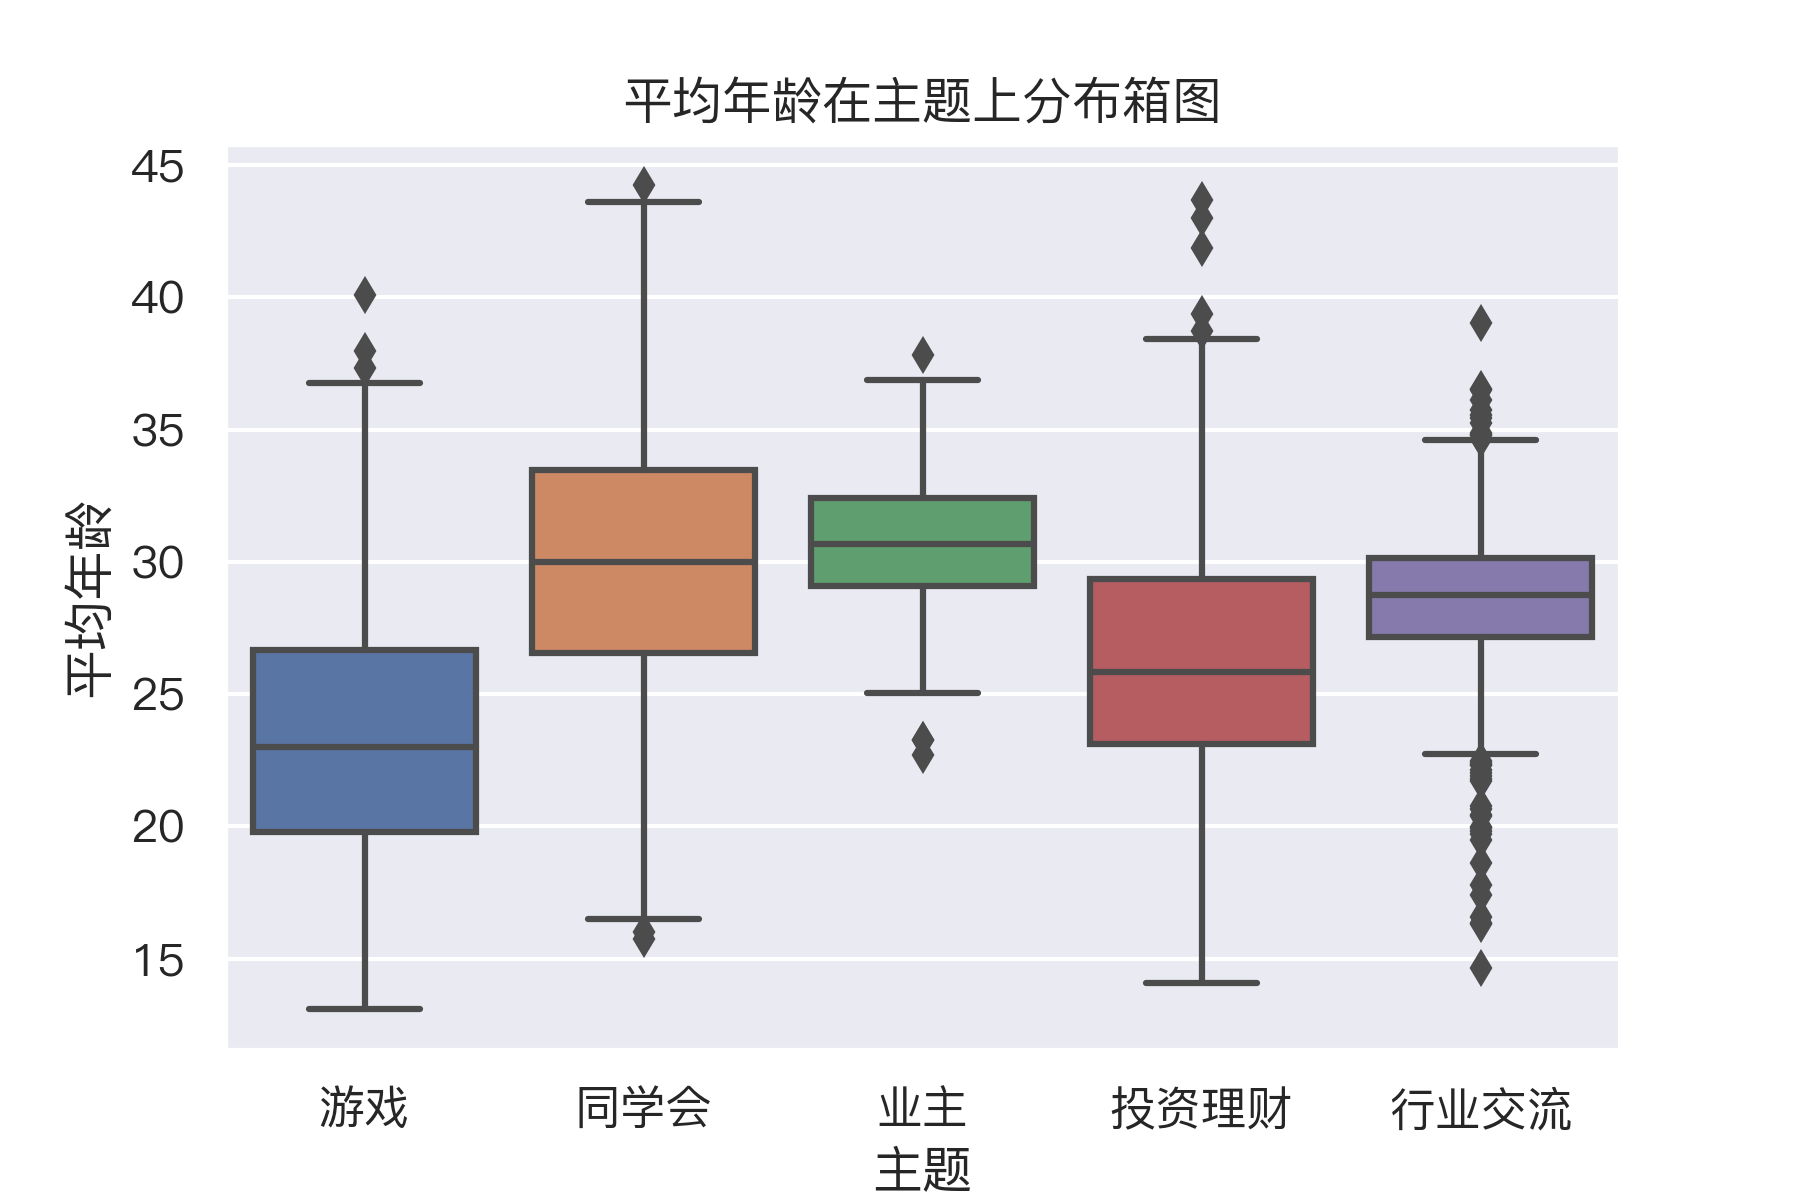
\includegraphics[width=0.95\textwidth]{task2-boxplot}
        \caption{平均年龄随主题变化统计观测}
        \label{fig:task2-boxplot}
    \end{figure}

    由此,我们将两个假设阐述如下:
    \begin{quote}
        H0:不同主题的群之间,平均年龄的分布无显著差异。

        H1:不同主题的群之间,平均年龄的分布差异显著。
    \end{quote}

    \section{任务3} % (fold)
    Use your favorite statistics analysis software, like Matlab, R, Excel, SPSS or ...
    \subsection{问题1} % (fold)
    \paragraph{问题描述} Draw the empirical probability density function of Col[7], i.e. the empirical pdf of average age. Does the data in this dimension follow Gaussian distribution? Test normality of Col[7].

    为平均年龄数据绘制直方图及经验概率密度函数,如\cref{fig:task3-pdf}所示。
    \begin{figure}[htbp]
        \centering
        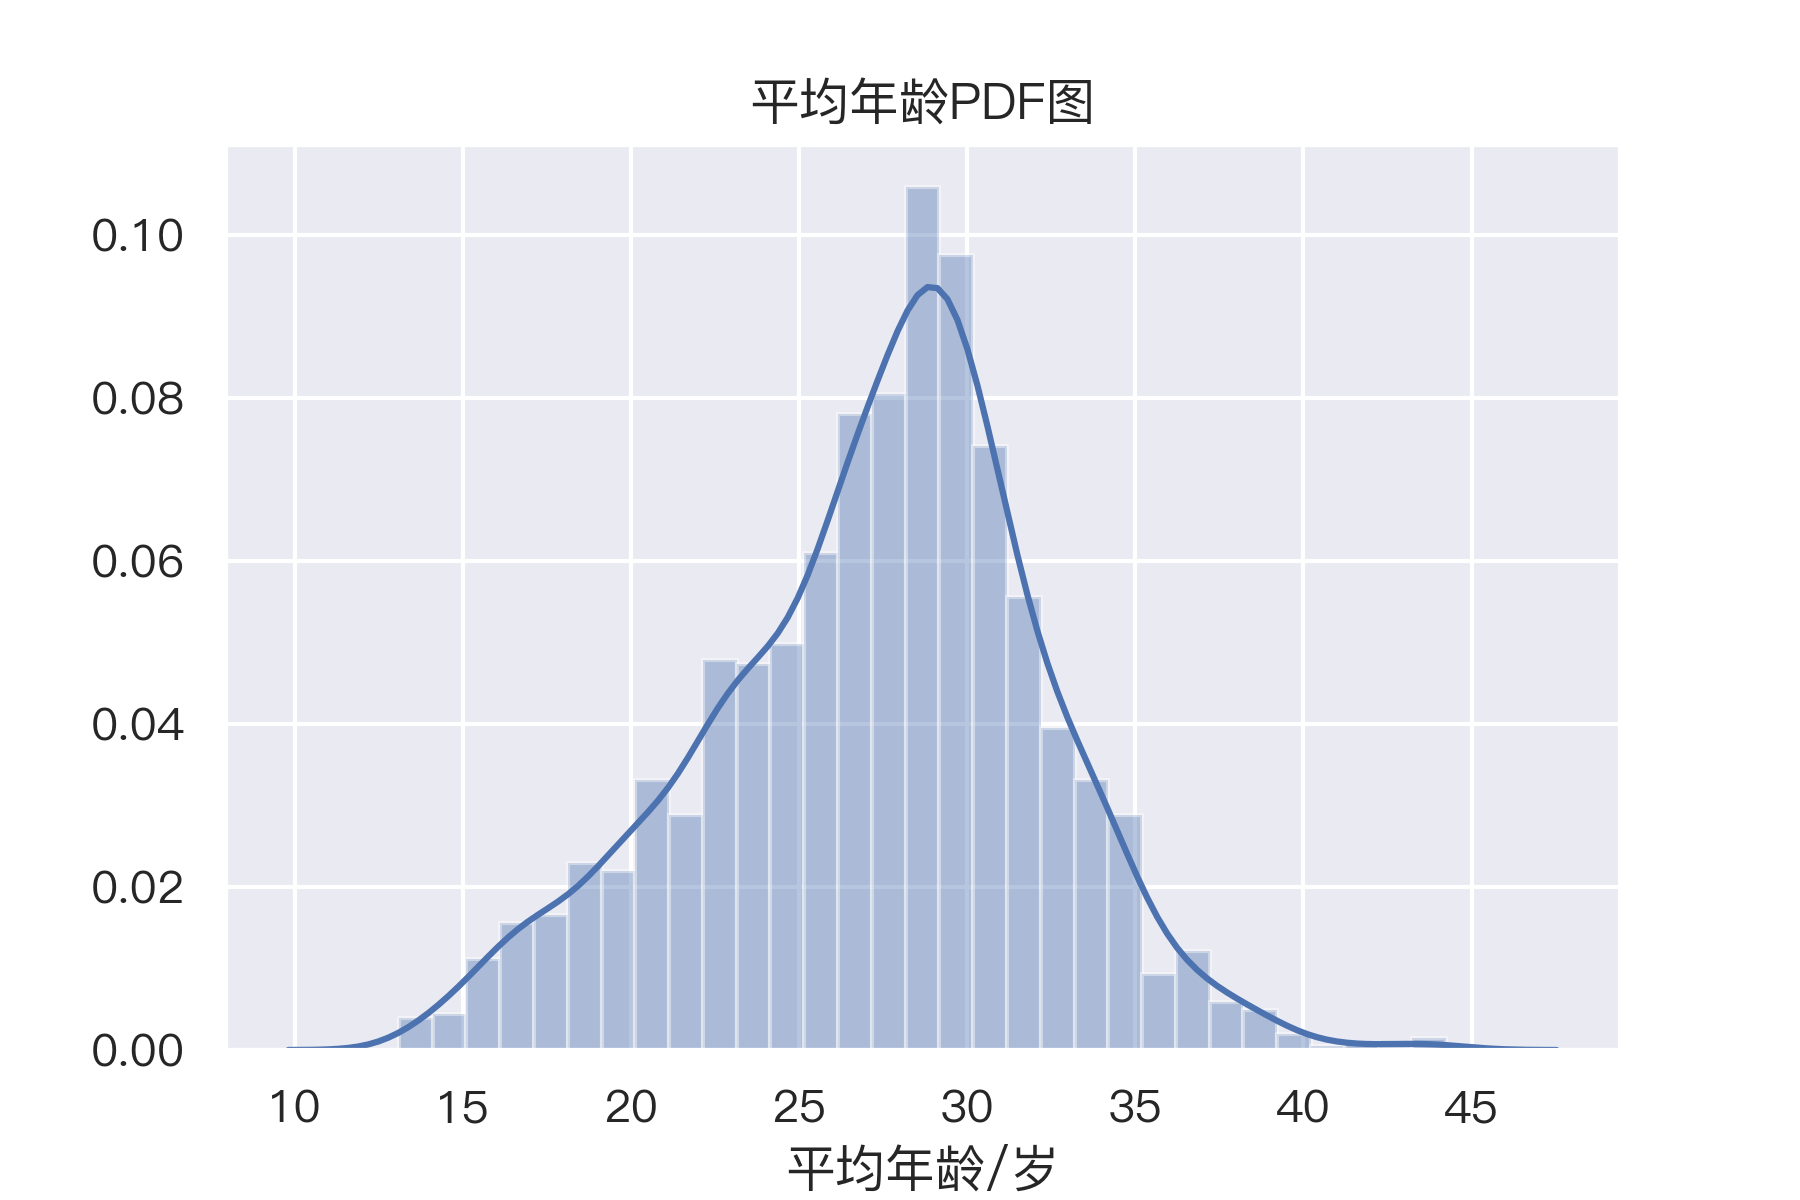
\includegraphics[width=0.95\textwidth]{task3-pdf}
        \caption{平均年龄经验概率密度函数}
        \label{fig:task3-pdf}
    \end{figure}

    可以看到,其相较于正态分布,曲线腰部更瘦,且有明显偏移。为了对该分布的正态性进行验证,可以利用课堂上提到的Skew and Kurtosis Test方法,即偏度-峰度检验。该检验的原假设为“被试分布具有正态性”,备择假设为“被试分布不具备正态性”。得到计算结果如\cref{task3q1log}所示。
    \lstinputlisting[label=task3q1log]{meta/task3q1.log}

    可见,在选取$\alpha=0.05$作为标准时,$pValue<\alpha=0.05$,即有充分把握拒绝原假设,因此该分布不满足正态性。

    \subsection{问题2} % (fold)
    \paragraph{问题描述} In Col[7], there are 5 components divided by category labels. We denote the data in Col[7] with category i (where i = 1,...,5) as Col[7| categoty=i]. Test the normality of each components and test the homogeneity of variances.

    分组后进行同样的检验操作,得到结果如\cref{task3q2log}。可以直接看出,类别编号1,4,5组的平均年龄不满足正态性,类别编号2、3的组可以认为满足正态性。
    \lstinputlisting[label=task3q2log]{meta/task3q2.log}

    对于方差齐的检验,应使用课程中提及的2倍标准差判据。对各组标准差进行计算,并取其中最大值、最小值进行比较,结果如\cref{task3std}。可见,同学会的平均年龄标准差是最大的,业主的平均年龄标准差是最小的。这个结论在\cref{fig:task2-boxplot}的箱图中也可以看出。另一方面,从社会经验上看,同学会存在于各个年龄段,而业主则主要是实现了积累的中老年,符合此处的结论。
    \lstinputlisting[label=task3std]{meta/task3std.log}

    对平均年龄而言,标准差最大值最小值之比,约为2(仅仅略大),此时我们可以认为该分部满足方差齐的条件。

    \subsection{问题3}
    \paragraph{问题描述} Do the one-way ANOVA test for Col[7] with categories in Col[2]. Write down your conclusion, supporting statistics, and visualize your data which inspire the process.

    利用F检验计算ANOVA,得到结果如\cref{tbl:task3q3}所示。注意到,$PR<\alpha=0.05$,因此有充分把握拒绝原假设。故结论是,不同主题的群之间,平均年龄的分布差异显著。
    \begin{table}
      \centering
      \caption{平均年龄-群类别ANOVA}
      \label{tbl:task3q3}
      \include{meta/task3q3}
    \end{table}
    TODO

    \section{任务4} % (fold)
    \paragraph{问题描述} Choose another 3 columns, draw the empirical pdf of each feature columns and test which column follows these assumptions in question 1? How about their corresponding log transformation?

    选取性别比、无回应比例以及图片比例三组特征,分别给出经验概率密度函数图像,如\cref{fig:gnn}所示。

    \begin{figure}[htbp]
        \centering
        \includegraphics[width=\textwidth]{task4-pdf}
        \caption{三组特征经验概率密度函数}
        \label{fig:gnn}
    \end{figure}

    针对以上三个特征的正态性进行检验,同样使用偏度-峰度法,得到结果如\cref{task4norm}。结果显示三组均不满足正态性。另外,结果也展示了方差齐检验的结果。无回应比例满足方差齐的条件,图片比例不满足方差齐的条件,而性别比的校验值略大于2,一定程度上可以近似认为满足方差齐。
    \lstinputlisting[label=task4norm]{meta/task4norm.log}

    对这三组数据进行对数变换,即$y=\log(x)$。注意到,$x=0$为奇异点,因此在实际应用中需要考虑零值的处理方式。首先,对所选数据的零值数量进行统计,得到如\cref{task4zerocount}的结果。
    \lstinputlisting[label=task4zerocount]{meta/task4zerocount.log}
    其中,性别比、无回应比的零值较少,而图片比例的零值较多。对于零值,我们有两种处理方法。
    \paragraph{方案1} 给所有值加上一个小量,如$10^{-6}$,然后进行对数变换。由于该调整量很小,因此不影响整体的分布情况。

    如果采用方案1,求得的概率密度函数如\cref{fig:task4loggnn}所示,相应的正态性检验结果如\cref{task4lognorm}所示,可见,三组数据的对数变换均不满足正态性。图片比例的对数变换满足方差齐,而其他两个特征不满足方差齐。

    \begin{figure}
      \includegraphics[width=\textwidth]{task4-logpdf}
      \caption{三组特征对数变换概率密度函数}
      \label{fig:task4loggnn}
    \end{figure}

    \lstinputlisting[label=task4lognorm]{meta/task4lognorm.log}
    \paragraph{方案2} 直接忽略零值,求取其他数值的对数变换。如果零值较少,可以认为其为毛刺点而将其忽略。

    如果采用方案2,求得的概率密度函数如\cref{fig:task4loggnn}所示,相应的正态性检验结果如\cref{task4lognorm0}所示。可见,性别比、无回应比例的对数变换均不满足正态性。其中,图片比例并不适宜采用本方案,但即便采用,依然没有正态性。无回应比例在此处满足方差齐,而性别比则不满足方差齐。

    \lstinputlisting[label=task4lognorm0]{meta/task4lognorm0.log}

    从以上统计结果及图像中均可以看到,性别比的经验概率密度分布比较接近正态,图片比例去零取对数后的经验概率密度分布比较接近正态。然而,这两种情况均未通过正态性检验,我们并没有充分的把握说明其正态性,且图片比例数据并不适宜去零处理。
    \section{任务5} % (fold)
    How to do one-way ANOVA with the non-normal data?
    \subsection{问题1} % (fold)
    \paragraph{问题描述} Find and list the possible solutions set.
    \begin{enumerate}
      \item One-way ANOVA对于正态性假设来说是鲁棒的,样本的费正态性对Type-I错误的影响较小,因此可以依然使用One-way ANOVA算法。
      \item 使用非参数Kruskal-Wallis H检验。
    \end{enumerate}

    H检验不需要各样本总体为正态分布,常被用于检验多个总体的分布是否存在显著差异。其原假设是: 多个独立样本来自的多个总体的分布无显著差异,备择假设则是多个总体的分布有显著差异。多独立样本 Kruskal-Wallis 检验的基本思想是:首先,将多组样本数混合并按升序 排序,求出各变量值的秩;然后,考察各组秩的均值是否存在显著差异。 如果各组秩的均值不存在显著差异, 则认为多组数据充分混合,数值相差不大,可以认为多个总体的分布无显著差异;反之,如果各组秩的均值存 在显著差异,则是多组数据无法混合,有些组的数值普遍偏大,有些组的数值普遍偏小,可认为多个总体的分 布存在显著差异,至少有一个样本不同于其他样本。[TODO ref]

    K-W统计量可表达为\cref{eq:kw},随后可用卡方分布获得置信概率。
    \begin{equation}
      \label{eq:kw}
      KW = \frac{12}{n(n+1)}\sum_{i=1}^k{\frac{R_i^2}{n_i}-3(n+1)}
    \end{equation}
    \subsection{问题2}
    \paragraph{问题描述} Do the one-way ANOVA on the 3 columns you choose. Do these feature columns vary significantly? Visualize the results.

    采用非参数的Kruskal-Wallis检验法,对三种特征进行检验,结果如\cref{task5kwtest}所示。可见,检验均拒绝了原假设,因此我们有充分的把握,说明对于这三种特征而言,五种类别是有显著区别的。
    \lstinputlisting[label=task5kwtest]{meta/task5kwtest.log}

    从\cref{fig:violin3}中可以看出,对于每一组特征,五个类别的分布函数不尽相同,因此也可以直观看出他们有显著区别。
    \begin{figure}
      \includegraphics[width=\textwidth]{task5-boxplot}
      \caption{三组特征小提琴图}
      \label{fig:violin3}
    \end{figure}

    \section{任务6} % (fold)
    \paragraph{问题描述} Redo the ANOVA test in question 3 c) by sampling 10\% data (i.e. around 200 groups). Repeat 10 times and compute the mean and standard deviation of the supporting statistics (F value). Compare at least two sampling strategies. Which sampling method is more stable? How are the results compared to the results without sampling? Why?

    给出四种抽样策略:
    \begin{enumerate}
      \item 随机抽样(rand):产生一组随机序号,以此选出10\%的样本。
      \item 分层抽样(group):依据原样本中的类别,在各个类别中随机抽样,抽样数为原类别样本数的10\%。
      \item 基于权重的抽样(weight):以每个群的总人数作为权重,将各权重之和归一化后作为选中概率。这种抽样方法的目的,是为了尽量保存群人数多的群,我们认为这一类群在体现比例特征时更有代表性。
      \item 分层权重抽样(group-weight):即在依据类别分层的同时,也依据群人数权重决定选中概率。
    \end{enumerate}

    利用以上4种抽样策略,重做对平均年龄的ANOVA。为了进一步验证抽样策略的有效性,此处还对前文所选的另外三个特征重做ANOVA。分别计算10次得到一组F值,按照题目要求计算均值和方差,结果分别如\cref{tbl:task6-fmean, tbl:task6-fvar}所示。

    \begin{table}[htbp]
      \centering
      \caption{不同抽样策略下不同特征ANOVA-F值平均值}
      \label{tbl:task6-fmean}
      \include{meta/task6-fmean}
    \end{table}
    \begin{table}[htbp]
      \centering
      \caption{不同抽样策略下不同特征ANOVA-F值方差}
      \label{tbl:task6-fvar}
      \include{meta/task6-fvar}
    \end{table}

    为了更直观地看出不同抽样方法的稳定性,可以将F值方差结果分别在不同特征上标准化,并作出柱状图,如\cref{fig:task6-fvar}所示。注意,由于经过了标准化,因此图中不同特征之间的柱无可比性,而实际上比较不同特征的F值方差也是没有意义的。从图中可以看到,在平均年龄上,随机抽样的稳定性表现较好,有更低的方差。但在其他的特征上,随机抽样未必会一直有良好的稳定性。例如,性别比特征中,分层权重抽样表现较好。

    \begin{figure}[htbp]
      \includegraphics{task6-fvar}
      \caption{F值方差对比}
      \label{fig:task6-fvar}
    \end{figure}

    TODO 和无抽样的对比

    \section{任务7} % (fold)
    \paragraph{问题描述} Choose any two categories, and classify them by logistical regression, or you can try multi-label classification on all categories.
    所谓Logistics Regression,是指一种基于Logistics函数的广义线性回归。Logistics函数又称Sigmoid函数,表达式如\cref{eq:sigmoid}所示。【TODO:ref】
    \begin{equation}
      \label{eq:sigmoid}
      \sigma(z) = \frac{1}{1+e^{-z}}
    \end{equation}

    Sigmoid函数是连续可微的函数,它可以将任意的$z$值映射到0和1附近,类似于阶跃函数。这种特性使得Sigmoid函数广泛应用于分类当中。函数图像如\cref{fig:sigmoid}所示,可以看到,该图像近似在0附近阶跃。
    \begin{figure}
      \includegraphics{task7-sigmoid}
      \caption{Sigmoid函数图像}
      \label{fig:sigmoid}
    \end{figure}

    若以$h_\theta(x)$代表特征变量$x$对应分类$y=1$的概率,则分类$y=0$的概率为$1-h_\theta(x)$。故可将概率函数表达为\cref{eq:lr_poss}。
    \begin{equation}
      \label{eq:lr_poss}
      \begin{aligned}
        h_\theta(x) &= 1-\frac{1}{1-e^{-\theta^T x}} \\
        P(y|x;\theta) &= (h_\theta(x))^y (1-h_\theta(x))^{1-y}
      \end{aligned}
    \end{equation}

    由于$n$个样本相互独立,则联合分布可以表示为各边际分布的乘积,似然函数可表示为\cref{eq:l}。
    \begin{equation}
      \label{eq:l}
      L(\theta) = \prod_{i}^n {P(y^{(i)}|x^{(i)};\theta)} = \prod_{i}^n {(h_\theta(x^{(i)}))^{y^{(i)}} (1-h_\theta(x^{(i)}))^{1-y^{(i)}}}
    \end{equation}

    取似然函数的对数,得到\cref{eq:logl}。
    \begin{equation}
      \label{eq:logl}
      l(\theta) = \log(L(\theta)) = \sum_{i}^n {y^{(i)} \log(h_\theta(x^{(i)})) + (1 - y^{(i)}) \log(h_\theta(1-x^{(i)}))}
    \end{equation}

    应用极大似然法,使用梯度下降求解问题$\min^{\theta} l(\theta)$即可求得一组参数$\theta^*$。

    对于本问题,任选两个类别的群,应用Logistic Regression及SVM(Support Vector Machine)算法进行预测。SVM算法在多维分类问题上往往有出色的表现,近年来被广泛应用,此处作为对比。其中训练样本比例取为0.9,测试样本比例选为0.1。预测准确率统计如\cref{task7-two}所示。根据结果可见,在不同的类别之间,Logistics回归算法与SVM算法的表现均有所变化,且变化趋势相近,范围大致在75\%-95\%之间变化。同时,不同的类别组合下,Logistics回归与SVM各有优劣,总体上SVM算法更加稳定。
    \lstinputlisting[label=task7-two]{meta/task7-two.log}

    尝试同时辨别5种类别的群,采用同样的样本划分方式,预测准确率如\cref{task7-multi}所示。此处可见,SVM算法在多类别划分上更有优势。
    \lstinputlisting[label=task7-multi]{meta/task7-multi.log}
    \label{applastpage}
    \newpage
    \bibliography{report}
    \bibliographystyle{unsrt}
\iffalse
\begin{itemize}[noitemsep,topsep=0pt]
%no white space
\end{itemize}
\begin{enumerate}[label=\Roman{*}.,noitemsep,topsep=0pt]
%use upper case roman
\end{enumerate}
\begin{multicols}{2}
%two columns
\end{multicols}
\fi
\end{document}
